\documentclass[
  parskip=half,           % halbzeiliger Zeileneinzug nach Absatz
  bibliography=totoc,     % Literatur im Inhaltsverzeichnis
  captions=tableheading,  % Tabellenüberschriften
  titlepage=firstiscover, % Titelseite ist Deckblatt
]{scrartcl}

\usepackage{geometry}
\geometry{a4paper,left=25mm,right=25mm, top=3cm, bottom=3cm}

% Paket float verbessern
\usepackage{scrhack}

% Warnung, falls nochmal kompiliert werden muss
\usepackage[aux]{rerunfilecheck}

% deutsche Spracheinstellungen
\usepackage{polyglossia}
\setmainlanguage{german}

% unverzichtbare Mathe-Befehle
\usepackage{amsmath}
% viele Mathe-Symbole
\usepackage{amssymb}
% Erweiterungen für amsmath
\usepackage{mathtools}

% Fonteinstellungen
\usepackage{fontspec}
% Latin Modern Fonts werden automatisch geladen

\usepackage[
  math-style=ISO,    % ┐
  bold-style=ISO,    % │
  sans-style=italic, % │ ISO-Standard folgen
  nabla=upright,     % │
  partial=upright,   % ┘
  warnings-off={           % ┐
    mathtools-colon,       % │ unnötige Warnungen ausschalten
    mathtools-overbracket, % │
  },                       % ┘
]{unicode-math}

% traditionelle Fonts für Mathematik
\setmathfont{Latin Modern Math}
\setmathfont{XITS Math}[range={scr, bfscr}]
\setmathfont{XITS Math}[range={cal, bfcal}, StylisticSet=1]

% Zahlen und Einheiten
\usepackage[
  locale=DE,                 % deutsche Einstellungen
  separate-uncertainty=true, % immer Fehler mit \pm
  per-mode=reciprocal,       % ^-1 für inverse Einheiten
  % alternativ:
  % per-mode=reciprocal, % m s^{-1}
  % decimal-marker=., % . statt , f�r Dezimalzahlen
]{siunitx}

% chemische Formeln
\usepackage[
  version=4,
  math-greek=default, % ┐ mit unicode-math zusammenarbeiten
  text-greek=default, % ┘
]{mhchem}

% tikzpicture ("Zeichenprogramm")
\usepackage{tikz}
\usetikzlibrary{circuits.ee.IEC}
\usetikzlibrary{positioning}
\tikzset{
  Pfeil/.style={thick,shorten >=#1,shorten <=#1,->,>=latex}, % für Peile
  UPfeil/.style={blue,Pfeil=#1,font={\sffamily\itshape}},% für Spannungspfeile
  IPfeil/.style={red,Pfeil=#1,font={\ttfamily\itshape}} % für Strompfeile
}
%Volt- und Amperemeter festlegen:
\tikzset{circuit declare symbol = Us}
\tikzset{set Us graphic ={draw,generic circle IEC, minimum size=5mm,info=center:$U_s$}}

\tikzset{circuit declare symbol = voltmeter}
\tikzset{set voltmeter graphic ={draw,generic circle IEC, minimum size=5mm,info=center:V}}

% richtige Anführungszeichen
\usepackage[autostyle]{csquotes}

% schöne Brüche im Text
\usepackage{xfrac}

\usepackage{blindtext}    % \blindtext zum Testen von Texten.

% Standardplatzierung für Floats einstellen
\usepackage{float}
\floatplacement{figure}{htbp}
\floatplacement{table}{htbp}

% Floats innerhalb einer Section halten
\usepackage[
  section, % Floats innerhalb der Section halten
  below,   % unterhalb der Section aber auf der selben Seite ist ok
]{placeins}

% Seite drehen für breite Tabellen
\usepackage{pdflscape}

% mehrere Seiten einer einzelnen pdf, zB
% \includepdf[pages={1-2}]{Bilder/Messdaten.pdf}
\usepackage{pdfpages}

% Captions schöner machen.
\usepackage[
  labelfont=bf,        % Tabelle x: Abbildung y: ist jetzt fett
  font=small,          % Schrift etwas kleiner als Dokument
  width=0.9\textwidth, % maximale Breite einer Caption schmaler
  %indention=1cm        % Einrückung nach der ersten Zeile
]{caption}
% subfigure, subtable, subref
\usepackage{subcaption}

% mit Buchstabend gelistete items: \begin{enumerate}[label={\alph*)}]
\usepackage{enumitem}

% Grafiken können eingebunden werden
\usepackage{graphicx}
% größere Variation von Dateinamen möglich (Probleme mit Leerzeichen behoben)
\usepackage{grffile}

% schöne Tabellen
\usepackage{booktabs}
\sisetup{table-format=1.2}
%\begin{tabular}{S[table-format=3.0] S S S S[table-format=3.2]}
%table-format : 3 stellen vor, 0 stellen nach dem Komma
% S steht f�r siunix, dh. wir verwenden solche Zahlen
% \multicolumn{2}{c}{Spalte 1}
% wie in excel Spalten zusammenf�gen
% Einheiten: {$\lambda \:/\: \si{\nano\meter}$}

% Uncertainties:
%\begin{tabular}{
% S[table-format=3.1]
% @{${}\pm{}$}
% S[table-format=2.1]
% }
% \toprule
% \multicolumn{2}{c}{$x \:/\: \si{\ohm}$} \\
% \midrule
% 632.4 & 5.7 \\

% Verbesserungen am Schriftbild
\usepackage{microtype}

% Literaturverzeichnis
\usepackage[
  backend=biber,
]{biblatex}
% Quellendatenbank
\addbibresource{Quellen.bib}
\addbibresource{programme.bib}

% Hyperlinks im Dokument
\usepackage[
  unicode,        % Unicode in PDF-Attributen erlauben
  pdfusetitle,    % Titel, Autoren und Datum als PDF-Attribute
  pdfcreator={},  % ┐ PDF-Attribute säubern
  pdfproducer={}, % ┘
  linkcolor=blue, % einfache interne Verkn?pfungen
  citecolor=blue, % Verweise auf Literaturverzeichniseintr?ge im Text
]{hyperref}
% erweiterte Bookmarks im PDF
\usepackage{bookmark}

% Trennung von Wörtern mit Strichen
\usepackage[shortcuts]{extdash}

\author{
  Johannes Kollek%
  \texorpdfstring{
    \\
    \href{mailto:johannes.kollek@udo.edu}{johannes.kollek@udo.edu}
  }{}%
  \texorpdfstring{\and}{, }
  Jean-Marco Alameddine%
  \texorpdfstring{
    \\
    \href{mailto:jean-marco.alameddine@udo.edu}{jean-marco.alameddine@udo.edu}
  }{}%
}
\publishers{TU Dortmund – Fakultät Physik}


% TYPOGRAPHIE:

% Nutze z.\,B. um Zeilenumbruch zu verhindern.
% Gedankenstriche mit --  (statt -)
% \\[2\baselineskip] erstellt einen vspace mit 2 Baselines, also 2 Zeilen


% \renewcommand{\baselinestretch}{1.3}										%Zeilenabstand


% zu breite Tabellen/Figures:
%\OverfullCenter{
%  \begin{figure}
%   ...
%  \end{figure}
%}
\NewDocumentCommand \OverfullCenter {+m} {
  \noindent\makebox[\linewidth]{#1} }



% Klammern werden nach außen hin leicht größer gesetzt.
\setlength{\delimitershortfall}{-1sp}


% Zusammenfassung neue Dinge: \Re(x)  \Im(x)  \v{x} \dif{x} \Dif{x}
% des weiteren werden in Mathebefehle.tex weitere Sachen definiert
% This work is licensed under the Creative Commons
% Attribution-NonCommercial 3.0 Unported License. To view a copy of this
% license, visit http://creativecommons.org/licenses/by-nc/3.0/.

% Differentialrechnung
\renewcommand{\d}{\ensuremath{\mathrm{d}}}

% Totale Ableitungen
\newcommand{\td}[2]{\ensuremath{\frac{\d{#1}}{\d{#2}}}}
\newcommand{\tdd}[2]{\ensuremath{\frac{\d^2{#1}}{\d{#2}^2}}}

% Partielle Ableitungen
\newcommand{\pd}[2]{\ensuremath{\frac{\partial{#1}}{\partial{#2}}}}
\newcommand{\pdd}[2]{\ensuremath{\frac{\partial^2{#1}}{\partial{#2}^2}}}

% Der Körper der reellen Zahlen
\newcommand{\R}{\ensuremath{\mathbb{R}}}

% Der Körper der natürlichen Zahlen
\newcommand{\N}{\ensuremath{\mathbb{N}}}

% Der Körper der komplexen Zahlen
\renewcommand{\C}{\ensuremath{\mathbb{C}}}

% Imaginäre Einheit
\newcommand{\iu}{{\mathrm{i}\mkern1mu}}

%Real- und Imaginärteil vernünftig mit \Re und \Im
\AtBeginDocument{ % wird bei \begin{document} ausgeführt
\let\symIm=\Im % werden sonst wieder von unicode-math überschrieben
\RenewDocumentCommand \Re {}
{
  \operatorname{Re}
}
\let\symIm=\Im
\RenewDocumentCommand \Im {}
{
  \operatorname{Im}
}
}


% mit \abs{x} und \norm{x} arbeiten
\DeclarePairedDelimiter{\abs}{\lvert}{\rvert}
\DeclarePairedDelimiter{\norm}{\lvert}{\rvert}


%\dif[x]{t}  : totale Ableitung von x nach t
\NewDocumentCommand \dif {O{leck mich} m}
{
  \frac{\mathinner{\symup{d} #1}} {\mathinner{\symup{d} #2}}
}

%\Dif{x}  : totale Ableitung von x
\NewDocumentCommand \Dif {m}
{
  \mathinner{\symup{D} #1}
}

% Mathemodus schönere Buchstaben mit \v{t}
\let\vaccent=\v % alten Befehl kopieren
\RenewDocumentCommand \v {} % Befehl überschreiben
{
  \TextOrMath{
    \vaccent % Textmodus
    }{
      \symbf
      }
}



\subject{Versuchsprotokoll zum Versuch Nr. 21}
\title{Optisches Pumpen}
\date{
  Durchführung: 15.05.2017
}

\begin{document}

\maketitle
\thispagestyle{empty}
\tableofcontents
\newpage

\section{Zielsetzung}


\section{Theorie}
\label{sec:Theorie}
\subsection{Allgemeine Theorie eines Reflexklystrons}
\label{sec:klysto}

Das Frequenzspektrum von Mikrowellen erstreckt sich von $\SI{300}{\mega\hertz}$ bis $\SI{300}{\giga\hertz}$.
In diesem Versuch wird zur Umwandlung von elektrischer in Mikrowellenenergie ein Reflexklystron benutzt.
Es handelt sich hierbei um eine Mikrowellenröhre, deren Aufbau in Abbildung \ref{fig:klystron} wiedergegeben ist.

\begin{figure}
  \centering
  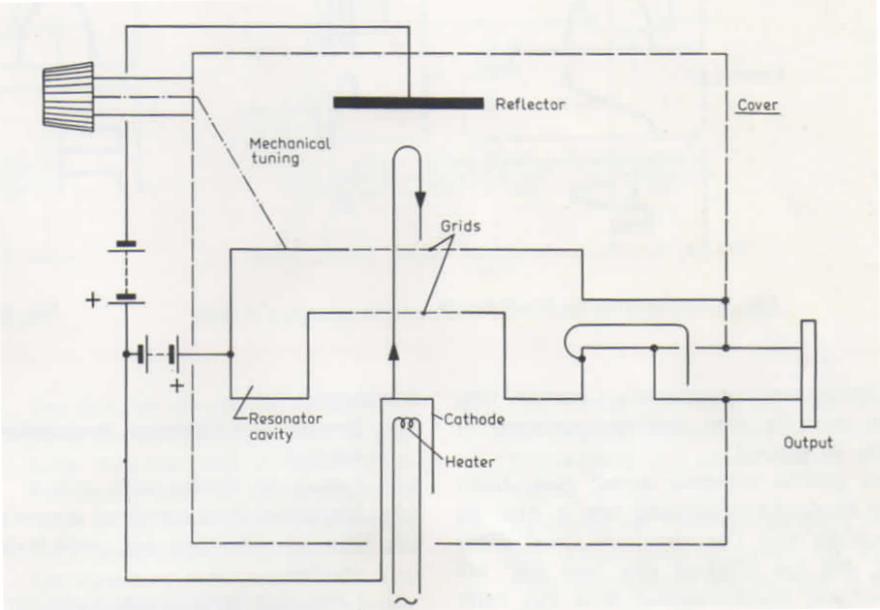
\includegraphics[height=8cm]{ressources/theorie.png}
  \caption{Schematischer Aufbau eines Klystrons \cite{skript}.}
  \label{fig:klystron}
\end{figure}

Es besteht hauptsächlich aus einem Glühdraht, einem Hochfrequenzresonator und einem Reflektor; letzterem verdankt es seinen Namen.
Aus dem Glühdrat werden Elektronen emittiert, welche zum Resonator beschleunigt werden.
Durchlaufen die Elektronen nun den Resonator, zwischen dessen Gittern ein Hochfrequenzfeld anliegt, tritt Geschwindigkeitsmodulation auf.
Diese ist in Abbildung \ref{fig:mod} dargestellt.

\begin{figure}
  \centering
  \begin{tikzpicture}
    \draw [->] (0,0) -- (0,4);
    \draw [->] (5,0.5) -- (5,0.75);
    \draw [->] (0,1) -- (10,1);
    \draw [->,red] (9,1) -- (9,4);
    \path node at (-0.25,4.25) {$V_{\text{HF}}$}
          node at (10.25,0.75) {$t$}
          node at (9.5,4.25)  {$\text{distance}$}
          node at (5,0.25) {$\frac{3}{4}T$};
    \draw (0,1) sin (1,2);
    \draw (1,2) cos (2,1);
    \draw (2,1) sin (3,0);
    \draw (3,0) cos (4,1);
    \draw (4,1) sin (5,2);
    \draw (5,2) cos (6,1);
    \path node at (1,0.75) {$A$}
          node at (2,0.75) {$B$}
          node at (3,0.75) {$C$};
    \draw [red] (1,1) to[out=85,in=180] (3.5,4);
    \draw [red] (3.5,4) to[out=0,in=90] (5,1);
    \draw [red] (2,1) to[out=85,in=180] (3.75,3.5);
    \draw [red] (3.75,3.5) to[out=0,in=90] (5,1);
    \draw [red] (3,1) to[out=85,in=180] (4,3);
    \draw [red] (4,3) to[out=0,in=90] (5,1);
  \end{tikzpicture}
  \caption{Darstellung der Geschwindigkeitsmodulation.}
  \label{fig:mod}
\end{figure}

Elektronen, die zu einem früheren Zeitpunkt $A$ in das Hochfrequenzfeld eintreten, werden zusätzlich beschleunigt, wohingegen, welche die zu einem späteren Zeitpunkt $B$ kommen, verlangsamt werden.
Nach Passieren des Resonators werden die Elektronen am negativ geladenen Reflektor reflektiert und, bei richtig eingestellter Reflektorspannung, gelangen alle Elektronen zu dem selben Zeitpunkt wieder im Resonator an (bunching), an dem sie maximal abgebremst werden.
Dies findet immer bei $(n+3/4)$ der Periodendauer des Resonators statt.
Die maximale Abbremsung gewährleistet die effektivste Umwandlung in Strahlungsenergie, welche sich im Output wiederspiegelt.\\
Wird die Reflektorspannung nun durchmoduliert, ergibt sich der Zusammenhang von Frequenz und Output, wie er in Abbildung \ref{fig:output} zu sehen ist.

\begin{figure}
  \centering
  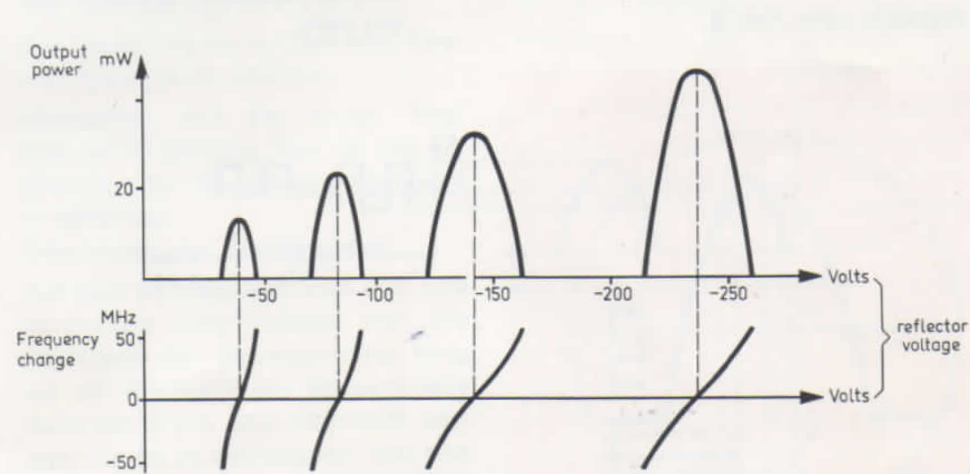
\includegraphics[height=6cm]{ressources/output.png}
  \caption{Typisches Signalbild des Versuchs \cite{skript}.}
  \label{fig:output}
\end{figure}

Es sind immer dann Peaks zu sehen, wenn die Reflektorspannung gerade so eingestellt ist, dass ein Elektronenbunch zum Zeitpunkt maximaler Abbremsung in den Resonator zurückkommt.
Ein Peak entspricht dabei einem Modus, welcher durch $(n+3/4)T$, der Aufenthaltsdauer der Elektronen im Resonatorraum, definiert ist.

\subsection{Wellen in einem Hohlleiter}

In dem Hohlleiter breiten sich die vom Klystron erzeugten Mikrowellen aus.
Die elektromagnetische Welle wird an jeder Unstetigkeit bzw nicht charakteristischen Impedanz im Leiter reflektiert.
Bei einer homogenen Leitung unendlicher Ausdehnung, sowie einer Leitung die mit einem Widerstand abgeschlossen ist der die charakteristische Impedanz der Leitung besitzt, treten keine Reflexionen auf.
Im Falle von Reflexionen ergibt sich die Feldstärke durch Addition der Amplituden der einlaufenden und reflektierten Welle, wobei die Amplitude und Phase letzterer von der Amplitude und Phase der reflektierenden Impedanz abhängen.
Durch die Addition bilden sich stehende Wellen im Leiter aus.
Maxima entstehen dort, wo sich die Wellen gleicher Phase addieren, bei Minima haben sie entgegengesetzte Phasen.
Der halbe Abstand zwischen zwei Maxima bzw. Minima definiert die Wellenlänge im Hohlleiter.
Für einen mit Luft gefüllten Hohlleiter gilt für die Wellenlänge
\begin{equation}
  \lambda_\text{g} = \frac{\lambda_0}{\sqrt{1-\left(\frac{\lambda_0}{\lambda_\text{c}}\right)^2}},
\end{equation}
wobei $\lambda_0$ die Wellenlänge im freien Raum und
\begin{equation}
  \lambda_\text{c} = 2a%\frac{2}{\sqrt{\left(\frac{m}{a}\right)^2 + \left(\frac{n}{b}\right)^2}}
\end{equation}
die kritische Wellenlänge für eine Halbwellen-Änderung in eine Richtung eines rechteckigen Hohlleiters mit Breite $a$ ist.
Daher gilt
\begin{equation}
  \lambda_0 = \frac{1}{\sqrt{\left(\frac{1}{\lambda_\text{g}}\right)^2+\left(\frac{1}{2a}\right)^2}} \label{eqn:1}
\end{equation}
und dadurch für die Frequenz
\begin{equation}
  f = \frac{c}{\lambda_0} = c \sqrt{\left(\frac{1}{\lambda_\text{g}}\right)^2+\left(\frac{1}{2a}\right)^2} \label{eqn:2}
\end{equation}
mit der Lichtgeschwindigkeit $c$ im freien Raum.

\subsection{Stehwellenverhältnis}
\label{sec:steh}

Das Stehwellenverhältnis bzw die Welligkeit $S$ ist das Verhältnis von maximaler und minimaler Feldstärke im Hohlleiter
\begin{equation}
  S = \frac{E_\text{max}}{E_\text{min}}.
\end{equation}
Es drei verschiedene Methoden die Welligkeit zu messen; die direkte, die "3 db-Methode" und die "Abschwächer-Methode".\\
Bei allen Methoden ist es üblich einen kleinen Teil der Leistung an der Leitung mit einer Sonde abzugreifen.
Das Signal wird an einen Detektor weitergegeben.
Bei der direkten Methode kann die Welligkeit direkt an einem SWR-Meter abgelesen werden.
Diese Methode ist jedoch nur genau bei kleinen Welligkeiten, da bei großen die Sondentiefe erhöht werden muss, was zu Störungen führt.
Die anderen beiden Methoden bieten dabei eine genauere Alternative.\\
Bei der "3 db-Methode" wird der Abstand zwischen zwei Punkten gemessen, an denen die Ausgangsspannung am Detektor den doppelten Wert des Minimums erreicht.
Die Welligkeit ergibt sich dann aus der Formel
\begin{equation}
  S = \sqrt{1+\frac{1}{\sin^2\left(\frac{\pi (d_1-d_2)}{\lambda_\text{g}}\right)}}, \label{eqn:3}
\end{equation}
wobei $d_1$ und $d_2$ die oben beschriebenen Punkte darstellen.\\
Bei der "Abschwächer-Methode" wird das Maximum am Detektor dem Minimum über Einstellen eines Dämpfungsgliedes gleichgemacht.
Dadurch folgt für die Welligkeit die Formel
\begin{equation}
  A_2-A_1 = 20\log(S), \label{eqn:4}
\end{equation}
dabei sind $A_1$ und $A_2$ die Einstellungen des Abschwächers vor und nach der Anpassung.
%\cite{skript}

% 2x2 Plot
% \begin{figure*}
%     \centering
%     \begin{subfigure}[b]{0.475\textwidth}
%         \centering
%         \includegraphics[width=\textwidth]{Abbildungen/Schaltung1.pdf}
%         \caption[]%
%         {{\small Schaltung 1.}}
%         \label{fig:Schaltung1}
%     \end{subfigure}
%     \hfill
%     \begin{subfigure}[b]{0.475\textwidth}
%         \centering
%         \includegraphics[width=\textwidth]{Abbildungen/Schaltung2.pdf}
%         \caption[]%
%         {{\small Schaltung 2.}}
%         \label{fig:Schaltung2}
%     \end{subfigure}
%     \vskip\baselineskip
%     \begin{subfigure}[b]{0.475\textwidth}
%         \centering
%         \includegraphics[width=\textwidth]{Abbildungen/Schaltung4.pdf}    % Zahlen vertauscht ... -.-
%         \caption[]%
%         {{\small Schaltung 3.}}
%         \label{fig:Schaltung3}
%     \end{subfigure}
%     \quad
%     \begin{subfigure}[b]{0.475\textwidth}
%         \centering
%         \includegraphics[width=\textwidth]{Abbildungen/Schaltung3.pdf}
%         \caption[]%
%         {{\small Schaltung 4.}}
%         \label{fig:Schaltung4}
%     \end{subfigure}
%     \caption[]
%     {Ersatzschaltbilder der verschiedenen Teilaufgaben.}
%     \label{fig:Schaltungen}
% \end{figure*}

\clearpage
\newpage
%\section{Fehlerrechnung}
Im folgenden Kapitel werden die wichtigsten Formeln der Fehlerrechnung aufgelistet, welche für die folgende Versuchsauswertung benötigt werden.
Der Mittelwert berechnet sich zu
\begin{equation}
  \overline{x} = \frac{1}{N} \sum_{i=1}^Nx_i
\end{equation}
Der Fehler des Mittelwertes berechnet sich zu
\begin{equation}
  \label{eq:std_mean}
  \Delta \overline{x} = \sqrt{\frac{1}{N(N-1)}\sum_{i=1}^N(x_i-\overline{x})^2}   \; .
\end{equation}
Die Schätzung der Standardabweichung berechnet sich zu
\begin{equation}
  \label{eq:std}
  \Delta x = \sqrt{\frac{1}{N-1}\sum_{i=1}^N(x_i-\overline{x})^2}     \; .
\end{equation}

Für die Fehlerrechnung wird bei allen folgenden Rechnungen das Gaußsche Fehlerfortpflanzungsgesetz
\begin{equation}
\increment{f} = \sqrt{\Bigl(\frac{\partial f}{\partial x_1}\increment{x_1}\Bigr)^2 + \Bigl(\frac{\partial f}{\partial x_2}\increment{x_2}\Bigr)^2 + \dotsc + \Bigl(\frac{\partial f}{\partial x_n}\increment{x_n}\Bigr)^2}
\end{equation}
für eine Funktion $f(x_1,x_2, \dotsc ,x_n)$, bei der die Größen $x_1, x_2, \dotsc , x_n$ voneinander unabhängig sind, verwendet.

Bei der linearen Regressionsrechnung gilt mit den Parametern $m$ und $b$ und der Ausgleichsgerade $y=mx+b$ der Zusammenhang:
\begin{align}
  m &= \frac{\overline{xy}-\overline{x}\cdot\overline{y}}{\overline{x²} - \overline{x}²} & &  b = \overline{y} - m \overline{x}  \; .
\end{align}
Dabei sind $x_i$ und $y_i$ linear abhängige Messgrößen. Der Fehler dieser Parameter errechnet sich zudem zu
\begin{align}
  \sigma_m^2 &= \frac{\sigma^2}{n(\overline{x²} - \overline{x}²)} & &\sigma_b^2 = \frac{\sigma^2\overline{x²}}{n(\overline{x²} - \overline{x}²)}
\end{align}
% Wenn Messdaten mit Vorhersagen verglichen werden sollen, benutzt man häufig die \emph{root mean square deviation}. Diese ist gegeben durch
% \begin{equation}
%   \label{eq:RMSE}
%   \textrm{RMSD} = \sqrt{\overline{(Y_\textrm{Messung}-Y_\textrm{Vorhersage})^2}}  \; .
% \end{equation}

%\clearpage
%\newpage
\section{Aufbau und Durchführung}
\subsection{Aufbau}
\label{sec:Aufbau}

Zur Bestimmung der Wärmekapazität eines Materials, im vorliegenden Fall Kupfer, soll der Probe eine fest definierte Wärmemenge zugeführt werden.
Dazu wird der in Abbildung \ref{fig:aufbau} skizzierte Versuchsaufbau verwendet.

\begin{figure}
  \centering
  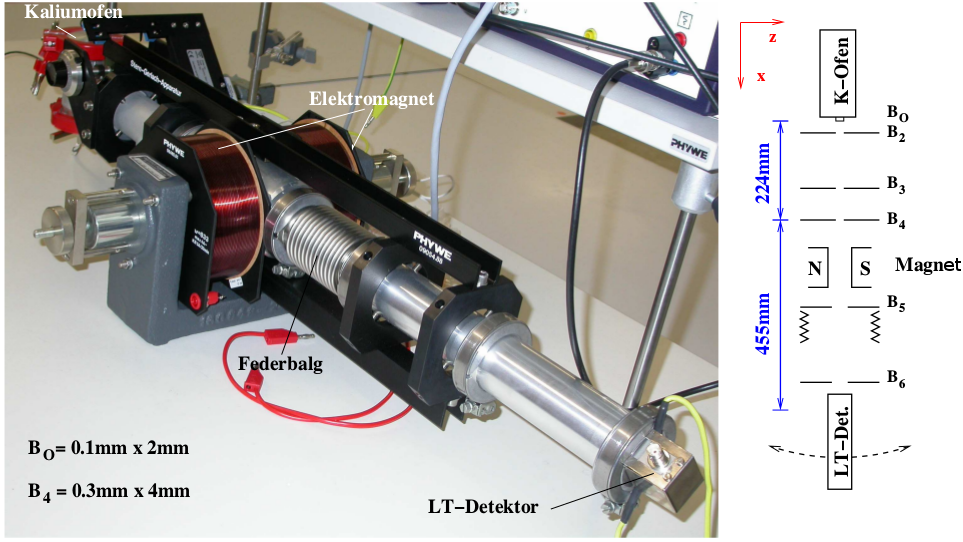
\includegraphics{ressources/aufbau.png}
  \caption{Skizze zum Versuchsaufbau.}
  \label{fig:aufbau} \cite{skript}
\end{figure}

Um dem Kupfer die Wärme zuzuführen, ist der Körper mit einer Heizwicklung umgeben.
Dessen Stromzufuhr wird über ein Konstantstromgerät geregelt, die Heizspannung wird zusätzlich über ein Voltmeter abgelesen.
Die Probe befindet sich in einem Kupferzylinder, welcher ebenfalls über eine Heizwicklung mit einer eigenen Stromversorgung verfügt.
Hierdurch kann gewährleistet werden, dass der Zylinder während des Versuches die gleiche Temperatur wie das Probematerial besitzt, um einen Wärmeaustausch zu vermeiden.

Der Kupferzylinder mit der Probe ist in einem Rezipienten, der mit einer Vakuumpumpe evakuiert werden kann.
Zusätzlich kann über ein Reduzierventil Gas, in unserem Fall Helium, aus einer Flasche in den Rezipienten geleitet werden.
Der Druck im Rezipienten wird dabei über ein Barometer festgehalten.

Der gesamte Rezipient wird über eine Halterung in ein Dewargefäß gehalten.
Dieses Dewargefäß besitzt zwei Wände, in dessem Zwischenraum ein Vakuum vorhanden ist.
Dies unterstützt die thermische Isolierung des Versuchsaufbaus, da das Vakuum einen maximal guten Isolator darstellt %duh
Zudem kann das Dewargefäß über einen Trichter mit flüssigem Stickstoff gefüllt werden, um die Probe zu kühlen.

Neben der festen Wärmezuführung muss auch die Temperatur, sowohl von der Probe als auch dem Kupferzylinder, gemessen werden.
Hierzu werden Ohmmeter, genauer Pt-100-Widerstände, als Widerstandsthermometer verwendet.
Diese Verwendung ist möglich, da der Widerstand von vielen Materialien, wie beispielsweise Platin, stark temperaturabhängig ist.
Die Umrechnung zwischen dem Widerstand und der Temperatur ist über eine monotone Funktion definiert, welche in der Auswertung angegeben wird.

%\clearpage
%\newpage
\subsection{Durchführung}
\label{sec:durchführung}
Bevor die eigentliche Durchführung der Versuchsteile beginnt, wird die Heizspannung für das Reflexklystron ca. 10 Minuten vor Versuchsbeginn eingestellt.

\subsubsection{Durchführung des ersten Versuchsteils}
Der Versuch wird wie in Abbildung \ref{sec:aufbau1} beschrieben aufgebaut.
Das Dämpfungsglied wird auf den passenden Wert für $\SI{30}{\decibel}$ eingestellt.
Die Reflektorspannung wird auf Wechselspannung gestellt und auf die x-Achse des Oszillographen gegeben, während das Signal des Detektors auf die y-Achse gegeben wird.
Hierdurch ergibt sich eine Kurve, die wie in Abbildung \ref{fig:output} dargestellt, eine Mode repräsentiert.

\begin{figure}
  \centering
  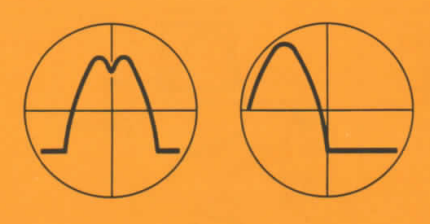
\includegraphics[height=5cm]{ressources/df1.png}
  \caption{Beobachtete Bodenkurve \cite{skript}. Links der durch den Frequenzmesser verursachte "Dip". Rechts die Messung der unteren Reflektorspannung. }
  \label{fig:df1}
\end{figure}

Die Reflektorspannung wird so gewählt, dass die Mitte der Mode mittig auf der x-Achse des Oszillographen liegt.
Zusätzlich wird die Mittenfrequenz bestimmt, indem der Frequenzmesser zu eingestellt wird, dass ein "Dip" in der Mitte der Mode zu sehen ist, wie es links in Abbildung \ref{fig:df1} dargestellt ist.
Die Mittenfrequenz, die passende Reflektorspannung sowie die Amplitude der Mode werden notiert.
Außerdem wird, wie in Abbildung \ref{fig:df1} rechts dargestellt, die untere sowie auch die obere Spannungsansatz-Spannung gemessen.
Dazu wird die Reflektorspannung so gewählt, dass sich ebendieses Bild ergibt.

Der gesamte Messvorgang wird für zwei weitere Moden wiederholt, welche in anderen Bereichen der Resonatorspannung zu finden sind.

Als weiterer Messprozess werden die Punkte der höchsten Mode gemessen, welche der vollen bzw. der halben Signalleistung entsprechen.
Hierzu wird die Mode über die Reflektorspannung vertikal jeweils auf die Mitte der Mode, den linken Punkt der mittleren Leistung bzw. auf den rechten Punkt der mittleren Leistung zentriert.
Die Frequenzen werden wiederum über den Frequenzmesser und den im Oszillographen beobachtbaren "Dip" ermittelt.
Die Reflektorspannungen sowie die Freuqenzen für die drei Punkte weden notiert.

\subsubsection{Durchführung des zweiten Versuchsteils}

Der Versuch wird wie in Abbildung \ref{sec:aufbau2} beschrieben aufgebaut, wobei zunächst der Abschluss eingebaut wird.

Das Reflexklystron wird mit einer Rechteck-Spannung moduliert Dämpfungsglied sowie Einstellung des SWR-Meters so gewählt, dass ein maximaler Ausschlag am SWR-Meter innerhalb des Skalenbereiches zu beobachten ist.
Es wird die im vorherigen Versuchsteil gefundene Mittenfrequenz der höchsten Mode verwendet.

Es wird nun der Abschluss durch den Kurzschluss ersetzt.
Mithilfe des Stehwellen-Detektors werden zwei Punkte minimalen Ausschlages am SWR-Meter gesucht und dessen Position notiert.

Zuletzt wird eine Dämpfungskurve aufgenommen, wozu der Kurzschluss am Hohlleiter wieder durch einen Abschluss ersetzt wird.
Das SWR-Meter wird so eingestellt, dass es bei einer vorgegebenen Einstellung durch das Dämpfungsglied einen maximalen Ausschlag von $\SI{0}{\decibel}$ anzeigt.
Die Dämpfung wird nun verstärkt, bis jeweils ein Ausschlag von $\SI{2}{\decibel}, \SI{4}{\decibel}, \SI{6}{\decibel}, \SI{8}{\decibel}, \SI{10}{\decibel}$ am SWR-Meter abzulesen ist.
Die Einstellungen des Dämpfungsgliedes an diesen Punkten werden notiert.

\subsubsection{Durchführung des dritten Versuchsteils}

Der Versuch wird wie in Kapitel \ref{sec:aufbau3} beschrieben aufgebaut.
Das Reflexklystron bleibt bei der im vorherigen Versuchsteil gewählten Einstellung.
Es sollen die Stehwellenverhältnissen mit den in Kapitel \ref{sec:steh} umschriebenen Methoden bestimmt werden.

Die erste Methode wird für die Einstellungen des Gleitschraubentransformators von $\SI{3}{\milli\metre}$, $\SI{5}{\milli\metre}$ und $\SI{7}{\milli\metre}$ durchgeführt.
Der Stehwellendetektor wird so platziert, dass das SWR-Meter ein maximales Signal detektiert.
Dieses Signal wird durch die Einstellung des SWR-Meters auf $\num{1.0}$ normiert.
Daraufhin wird die Sonde in ein Minimum verschoben und der Wert des SWR-Meters dort gemessen.

Bei der zweiten Methode, der "3 dB-Methode", wird der Gleitschraubentransformator auf $\SI{9}{\milli\metre}$ eingestellt, was einem höheren Stehwellenverhältnis entspricht.
Die Messsonde wird vertikal bewegt, bis sich ein Minimum am SWR-Meter ergibt.
Dieses wird auf einen Wert von $\SI{3}{\decibel}$ normiert.
Die Sonde wird nun einmal nach rechts und einmal nach links bewegt, bis sich ein Wert von $\SI{0}{\decibel}$ auf dem SWR-Meter ergibt.
Diese Werte werden notiert.

Zum Schluss wird die "Abschäwcher-Methode" genutzt, wobei auch hier der Gleitschraubentransformator auf $\SI{9}{\milli\metre}$ eingestellt wird.
Wiederum wird die Sonde vertikal bewegt, bis das SWR-Meter ein Minimum anzeigt.
Darufhin wird das Dämpfungsglied auf $\SI{20}{\decibel}$ eingestellt und die Einstellungen am SWR-Meter so gewählt, dass dort ein Wert von $\SI{3}{\decibel}$ angezeigt wird.
Die Sonde wird nun vertikal bewegt, bis das Signal ein relatives Maximum anzeigt.
Das Dämpfungsglied wird an dieser Stelle so verstellt, dass das SWR-Meter wieder $\SI{3}{\decibel}$ anzeigt.
Die Dämpfungsgliedeinstellung wird notiert.

\clearpage
\newpage
\section{Auswertung}
\label{sec:Auswertung}

% % Examples
% \begin{equation}
%   U(t) = a \sin(b t + c) + d
% \end{equation}
%
% \begin{align}
%   a &= \input{build/a.tex} \\
%   b &= \input{build/b.tex} \\
%   c &= \input{build/c.tex} \\
%   d &= \input{build/d.tex} .
% \end{align}
% Die Messdaten und das Ergebnis des Fits sind in Abbildung~\ref{fig:plot} geplottet.
%
% %Tabelle mit Messdaten
% \begin{table}
%   \centering
%   \caption{Messdaten.}
%   \label{tab:data}
%   \sisetup{parse-numbers=false}
%   \begin{tabular}{
% % format 1.3 bedeutet eine Stelle vorm Komma, 3 danach
%     S[table-format=1.3]
%     S[table-format=-1.2]
%     @{${}\pm{}$}
%     S[table-format=1.2]
%     @{\hspace*{3em}\hspace*{\tabcolsep}}
%     S[table-format=1.3]
%     S[table-format=-1.2]
%     @{${}\pm{}$}
%     S[table-format=1.2]
%   }
%     \toprule
%     {$t \:/\: \si{\milli\second}$} & \multicolumn{2}{c}{$U \:/\: \si{\kilo\volt}$\hspace*{3em}} &
%     {$t \:/\: \si{\milli\second}$} & \multicolumn{2}{c}{$U \:/\: \si{\kilo\volt}$} \\
%     \midrule
%     \input{build/table.tex}
%     \bottomrule
%   \end{tabular}
% \end{table}
%
% % Standard Plot
% \begin{figure}
%   \centering
%   \includegraphics{build/plot.pdf}
%   \caption{Messdaten und Fitergebnis.}
%   \label{fig:plot}
% \end{figure}
%
% 2x2 Plot
% \begin{figure*}
%     \centering
%     \begin{subfigure}[b]{0.475\textwidth}
%         \centering
%         \includegraphics[width=\textwidth]{Abbildungen/Schaltung1.pdf}
%         \caption[]%
%         {{\small Schaltung 1.}}
%         \label{fig:Schaltung1}
%     \end{subfigure}
%     \hfill
%     \begin{subfigure}[b]{0.475\textwidth}
%         \centering
%         \includegraphics[width=\textwidth]{Abbildungen/Schaltung2.pdf}
%         \caption[]%
%         {{\small Schaltung 2.}}
%         \label{fig:Schaltung2}
%     \end{subfigure}
%     \vskip\baselineskip
%     \begin{subfigure}[b]{0.475\textwidth}
%         \centering
%         \includegraphics[width=\textwidth]{Abbildungen/Schaltung4.pdf}    % Zahlen vertauscht ... -.-
%         \caption[]%
%         {{\small Schaltung 3.}}
%         \label{fig:Schaltung3}
%     \end{subfigure}
%     \quad
%     \begin{subfigure}[b]{0.475\textwidth}
%         \centering
%         \includegraphics[width=\textwidth]{Abbildungen/Schaltung3.pdf}
%         \caption[]%
%         {{\small Schaltung 4.}}
%         \label{fig:Schaltung4}
%     \end{subfigure}
%     \caption[]
%     {Ersatzschaltbilder der verschiedenen Teilaufgaben.}
%     \label{fig:Schaltungen}
% \end{figure*}



\input{build/Tabelle_messwerte.tex}

\input{build/Tabelle_ausdehnung.tex}

\clearpage
\newpage
\section{Diskussion}
\label{sec:Diskussion}

Für die ermittelten Debye-Temperaturen $\Theta_\text{D}$ haben sich die Werte
\begin{align*}
  \Theta_{\text{D,Exp}} &= \input{build/Theta_deb.tex} & \Theta_{\text{D,Theorie}} &= \input{build/Theta_deb_theo.tex}
\end{align*}
ergeben, was einer Abweichung des experimentellen Ergebnisses vom theoretisch errechneten Ergebnis nach dem Debye-Modell von
\begin{align*}
  \increment \Theta_\text{D} = \input{build/err_deb.tex}
\end{align*}
entspricht.
Dabei ist jedoch zu beachten, dass auch das Debye-Modell nur einer Näherung entspricht.
Dies spiegelt sich beispielsweise in der angenommenen linearen Dispersionsrelation wider.

Bei den experimentellen Werten fällt vor allem auf, dass sich die Wärmekapazität wider erwarten nicht gänzlich monoton mit der Temperatur verhält.
Dies kann auf systematische Fehler zurückgeführt werden, welche typisch für einen thermodynamischen Versuch sind:
Trotz Vakuum sind Wärmeverluste durch Wärmeleitung, Wärmestrahlung und Konvektion nicht gänzlich auszuschließen.
Zudem musste während des Versuches der umgebende Kupferzylinder ebenfalls auf der selben Temperatur wie die Probe gehalten werden.
Da dies nicht immer perfekt möglich war, treten auch hier Beeinflussungen durch Wärmezufuhr aus der zweiten Heizspule oder durch Wärmeabgabe an den Kupferzylinder auf.
Dies könnte auch eine Erklärung für das nicht-monotone Verhalten der Wärmekapazität darstellen.

Eine Fehlerquelle bei der Auswertung besteht in dem Sachverhalt, dass zur Bestimmung der Debye-Temperatur eine Tabelle mit festen Zahlenwerten verwendet wurde.
Durch Verwendung einer exakteren Tabelle, bzw. durch numerisches Ermitteln der jeweiligen Zahlenwerte, könnte die Genauigkeiten der Daten ebenfalls verbessert werden.\\
Abschließend lässt sich sagen, dass die durch die Messung ermittelten Werte relativ gut zu der in der Theorie beschriebenen Abhängigkeit von der Temperatur passen.

\clearpage
\newpage

\printbibliography

\clearpage
\newpage
\begin{appendix}


\section{Anhang}

\begin{figure}
  \centering
  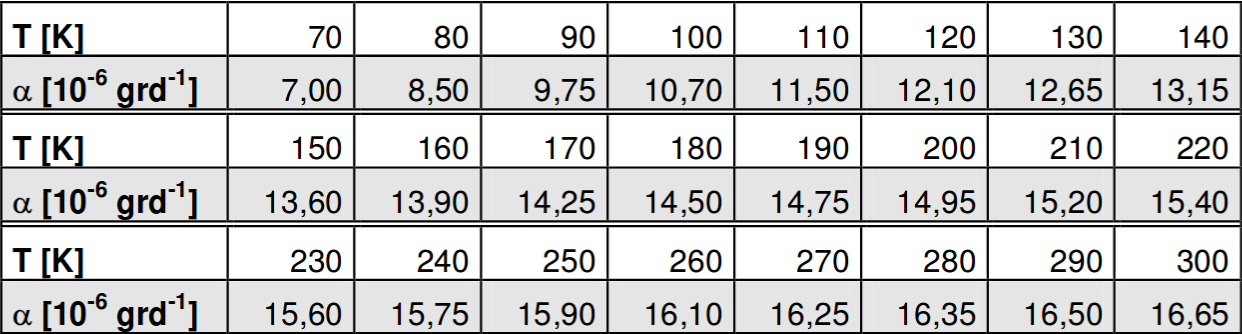
\includegraphics[width=\textwidth]{ressources/alpha.png}
  \caption{Ausdehnungskoeffizient $\alpha$ von Kupfer in Abhängigkeit von der Temperatur $T$. \cite{skript}}
  \label{fig:alphaa}
\end{figure}

\begin{figure}
  \centering
  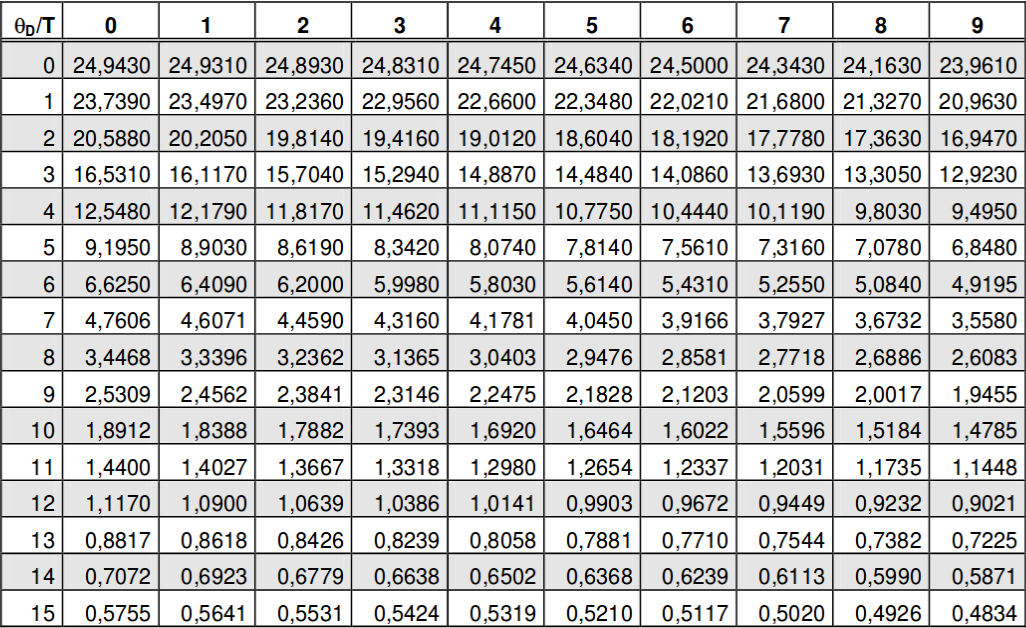
\includegraphics[width=\textwidth]{ressources/hugetable.png}
  \caption{Werte der Wärmekapazität aus der Debyefunktion in Abhängigkeit von der Debye-Temperatur $\Theta_\text{D}$ und der Temperatur $T$. \cite{skript}}
  \label{fig:mirfallenkeinelabelmehreinfuerdenganzenmistfuckthisshitimoutwarumtueichmirdasanundesistschonhalbzweinachtsdafuq}
\end{figure}
% \centering
% \begin{figure}
% \includepdf[width=0.9\textwidth, pages={1}]{Bilder/Messdaten.pdf}
% \end{figure}
% \newpage
% \begin{figure}
% \includepdf[width=0.9\textwidth, pages={2}]{Bilder/Messdaten.pdf}
% \end{figure}
%
\end{appendix}


\end{document}


% % Examples
% \begin{equation}
%   U(t) = a \sin(b t + c) + d
% \end{equation}
%
% \begin{align}
%   a &= \input{a.tex} \\
%   b &= \input{b.tex} \\
%   c &= \input{c.tex} \\
%   d &= \input{d.tex} .
% \end{align}
% Die Messdaten und das Ergebnis des Fits sind in Abbildung~\ref{fig:plot} geplottet.
%
% %Tabelle mit Messdaten
% \begin{table}
%   \centering
%   \caption{Messdaten.}
%   \label{tab:data}
%   \sisetup{parse-numbers=false}
%   \begin{tabular}{
%     S[table-format=1.3]
%     S[table-format=-1.2]
%     @{${}\pm{}$}
%     S[table-format=1.2]
%     @{\hspace*{3em}\hspace*{\tabcolsep}}
%     S[table-format=1.3]
%     S[table-format=-1.2]
%     @{${}\pm{}$}
%     S[table-format=1.2]
%   }
%     \toprule
%     {$t \:/\: \si{\milli\second}$} & \multicolumn{2}{c}{$U \:/\: \si{\kilo\volt}$\hspace*{3em}} &
%     {$t \:/\: \si{\milli\second}$} & \multicolumn{2}{c}{$U \:/\: \si{\kilo\volt}$} \\
%     \midrule
%     \input{table.tex}
%     \bottomrule
%   \end{tabular}
% \end{table}
%
% % Standard Plot
% \begin{figure}
%   \centering
%   \includegraphics{plot.pdf}
%   \caption{Messdaten und Fitergebnis.}
%   \label{fig:plot}
% \end{figure}
